\documentclass[useAMS, usenatbib, preprint, 12pt]{aastex}
\usepackage{cite, natbib}
\usepackage{float}
\usepackage{epsfig}
\usepackage{cases}
\usepackage[section]{placeins}
\usepackage{graphicx, subfigure}
\usepackage{color}
\usepackage{bm}

\newcommand{\columbia}{1}
\newcommand{\simons}{2}
\newcommand{\nyu}{3}
\newcommand{\cca}{4}
\newcommand{\mpia}{5}
\newcommand{\cds}{6}
\newcommand{\naigrain}{333}
\newcommand{\nmcquillan}{100}
\newcommand{\kepexample}{1430163}
\newcommand{\kepexampleperiod}{4}
\newcommand{\aigrainexampleperiod}{20.8}
\newcommand{\Kepler}{{\it Kepler}}
\newcommand{\kepler}{\Kepler}
\newcommand{\corot}{{\it CoRoT}}
\newcommand{\Ktwo}{{\it K2}}
\newcommand{\ktwo}{\Ktwo}
\newcommand{\TESS}{{\it TESS}}
\newcommand{\LSST}{{\it LSST}}
\newcommand{\Wfirst}{{\it Wfirst}}
\newcommand{\SDSS}{{\it SDSS}}
\newcommand{\PLATO}{{\it PLATO}}
\newcommand{\Gaia}{{\it Gaia}}
\newcommand{\gaia}{{\it Gaia}}
\newcommand{\Teff}{$T_{\mathrm{eff}}$}
\newcommand{\teff}{$T_{\mathrm{eff}}$}
\newcommand{\FeH}{[Fe/H]}
\newcommand{\feh}{[Fe/H]}
\newcommand{\ie}{{\it i.e.}}
\newcommand{\eg}{{\it e.g.}}
\newcommand{\logg}{log \emph{g}}
\newcommand{\dnu}{$\Delta \nu$}
\newcommand{\numax}{$\nu_{\mathrm{max}}$}
\newcommand{\acfRMS}{9.27}
\newcommand{\pgramRMS}{1.25}
\newcommand{\mcmcRMS}{0.46}
\newcommand{\racomment}[1]{{\color{red}#1}}

\begin{document}

\title{Investigating magnetic dynamo evolution with TESS field dwarfs}

\author{R. Angus\altaffilmark{\columbia, }\altaffilmark{\simons}
        J. R. Davenport, D. Busazi, D. Foreman-Mackey, A. Mann, S. Oh,
        D. Kipping
}

\altaffiltext{\columbia}{Department of Astronomy, Columbia University, NY, NY}
\altaffiltext{\simons}{Simons Fellow, RuthAngus@gmail.com}

\section{Introduction}

Among the key observable properties of main sequence stars in our Galaxy,
age is the most difficult to determine.
Traditionally, fitting isochrones to cluster stars was one of the only precise
methods for measuring ages but was extremely difficult for the majority of
isolated field stars, particularly for those without precise spectroscopic
information.
Methods such as asteroseismology and measuring Lithium abundances can provide
precise ages but require time intensive observations for each target and are
not capable of producing the large quantity of ages needed for exoplanet and
galactic population studies.

Galactic archaeology and exoplanet populations are two rapidly accelerating
fields of interest within astronomy. Although seemingly unconnected, these two
fields are linked by a mutual requirement for precise stellar parameters.
To galactic archaeologists, ages and elemental abundances are the most
important parameters.
Indeed, most galactic archaeology surveys target exactly these properties.
For exoplaneteers, masses and radii have historically been the most important
stellar parameters for understanding planetary systems.
With a growing number of planet hosts with precise masses and radii, attention
is turning toward other parameters such as ages to understand the history and
evolution of these systems.
Age is therefore a fundamental stellar parameter of great interest to two
large communities of astronomers.
However it is a difficult attribute to measure for main sequence F, G, K, and
M stars in the field, in part because low-mass dwarfs do not move far on the
Color-Magnitude diagram (CMD) during their hydrogen burning lifetimes.
Further, competing stellar evolution models predict different ages for the
same star.
Of the measurable properties for a large ensemble of field stars, rotation
periods contain the most information about stellar age, and provide the best
leverage for advancing our knowledge of galactic archeology as well as
exoplanet population demographics.

To improve our understanding of star and planet formation and evolution, as
well as the history of the Milky Way, we must constrain the ages of low-mass
stars like the Sun in the galactic field.
Fortunately nature has provided a powerful means to determine ages for main
sequence stars via their rotation.
Angular momentum is carried away though magnetically driven stellar winds,
which slows the star’s rotation over cosmic time. This rotation-based “clock”
is known as gyrochronology.
Cool spots on the star’s surface rotate in-to and out-of view, creating small
amplitude ($\pm$ 1\%) quasi-periodic changes in the stellar brightness.
While rotation periods have previously been measured from starspot-induced
flux modulations for hundreds of stars from the ground, space-based
photometric surveys have opened the door to homogeneous ensemble measures of
stellar rotation, and therefore age.
With precise light curves available from the TESS mission, we may be able to
determine rotation periods and ages for nearly 100,000 main sequence field
stars.

Additionally, rotation is related to stellar activity.
With so many TESS targets being M dwarfs which tend to be particularly active,
understanding the magnetic behavior of these stars has never been more
important.

To enable studies of stellar ages from rotation periods with TESS, we propose
to: 1. Measure accurate rotation periods for every available TESS FFI and
two-minute cadence target, using the most appropriate tools and methods
required.
2. Produce updated gyrochronology relations based on a wider range of field
star ages.
3. Determine the origin of the mysterious rotation period bimodality
discovered with Kepler by tracing the rotation period distribution over the
whole sky, and out to further distances utilizing public Gaia data.
4. Measure the star formation history across the sky using a new Bayesian
age-dating system.

\section{Scientific Justification}
\subsection{Rotation period bimodality}

\citet{McQuillan2014} demonstrated a striking discontinuity in the rotation
periods of Kepler M dwarfs.
They revealed a bimodal distribution of period, with a gap that depends on
mass.
Plenty of stars had rotation periods just shorter and just longer than this,
but very few had rotation periods around this value.
More recently, Davenport (2017) used Gaia data to elucidate this behaviour by
re-examining the Kepler rotation periods reported in McQuillan et al. (2014)
as a function of mass.
Davenport (2017) eliminated contaminating giants identified using Gaia
parallaxes, i.e. stars that are too bright to be
dwarfs given their distance.
These decontaminated data revealed that the period bimodality was not simply a
feature of M dwarfs but extended to the G and K stars.
Clearly then, this bimodal rotation period distribution is does not only
affect M dwarfs, but may be a feature of all stars, including the Sun.

\begin{figure}
\begin{center}
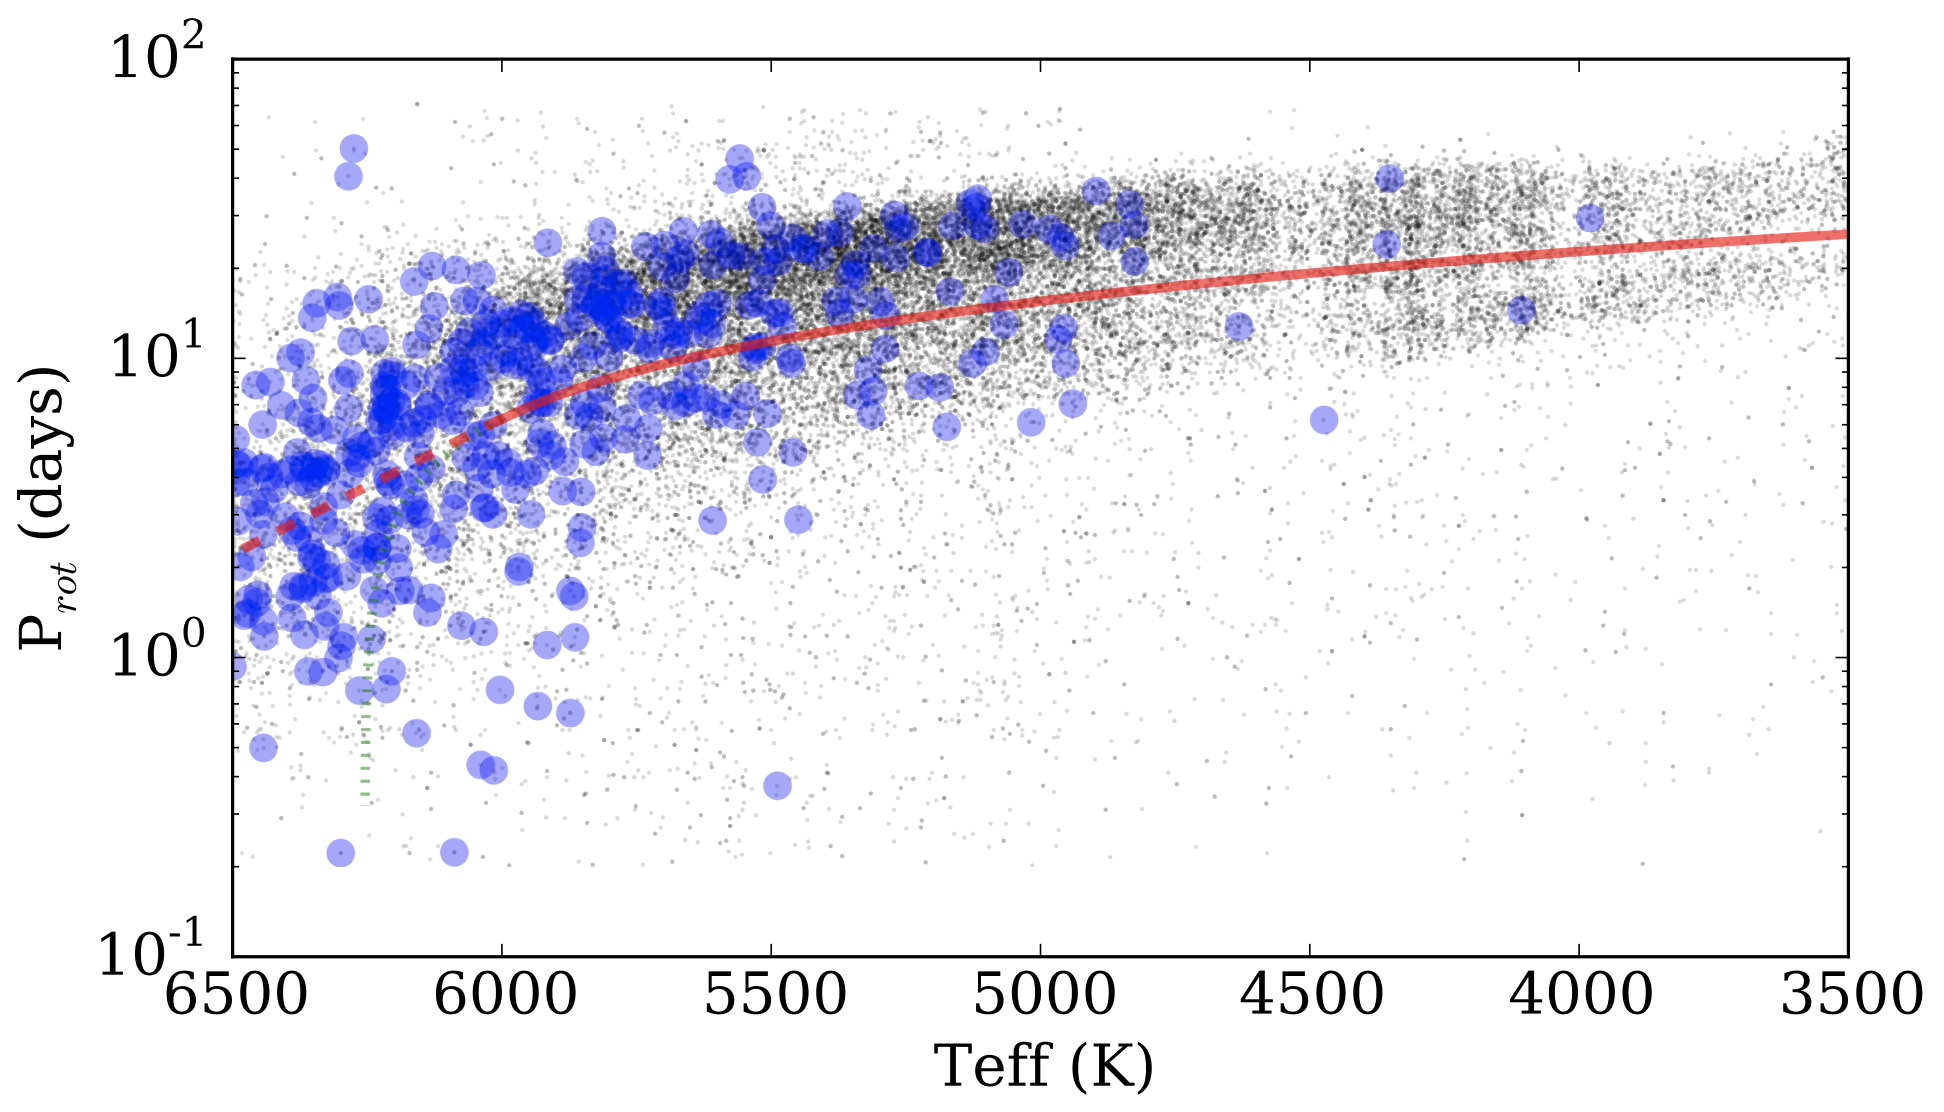
\includegraphics[width=3in, clip=true]{Davenport.png}
\caption{From Davenport (2017).
    Rotation period as a function of effective
temperature for the full McQuillan et al., (2014) Kepler sample in black, and
the subset of these stars that also feature in the TGAS Gaia DR1 catalogue in
blue. Contaminating giants have been removed from the blue sample and the
rotation period bimodality is revealed to exist across all temperatures shown.
    The red line is a 600 Myr rotational isochrone (also known as a gyrochrone).}
\label{fig:sip_hist}
\end{center}
\end{figure}

Intriguingly, the rotation gap is not constant across masses.
It appears at shorter rotation periods for more massive stars and longer
rotation periods for less massive stars.
In fact, it closely follows a contour of constant age, an isochrone of 600
Myr.
Two possible scenarios can explain this phenomenon.
The first is that stars undergo a transition in the behaviour of their
magnetic dynamo.
They switch from a fast to a slow rotating regime rapidly, spending little
time rotating at an intermittent period.
This transition would occur around 3-4 days for G dwarfs and 10-12 days for M
dwarfs.
Is this a convergence bump?
The rotation periods of stars are believed to have converged by around the age
of the Hyades, ~790 Myr (clusters younger than this show a broad spread in
rotation periods and older clusters a narrow one).
The age at which this transition occurs, around 600 Myr, is close to this.
Could this be a coincidence or do rotation periods undergo a rotation period
bump once they move stabilise onto a Skumanich spin-down regime?
If this is the case, a study of this transition could greatly advance our
understanding of the operation of stellar dynamos.

The rotation period bimodality seen in McQuillan et al. (2014) and Davenport
(2017) could also be explained by two waves of star formation: a short one
centered around a few hundred million years ago and a long one centered around
a few billion years ago.
TESS’s full view of the sky will allow us to establish the spatial extent of
this rotation period gap and investigate the underlying cause.

\subsection{Gyrochronology}

Gyrochronology is an active area of interest in astronomy today due to its applicability to stellar, exoplanet and galactic astronomy.
It is a method of age-dating stars that doesn’t require expensive
spectroscopy, requiring only a rotation period and a colour or temperature.
Considering the vast number of light curves that will be made available by
future photometric surveys, as well as the already formidable number produced
by the Kepler spacecraft, gyrochronology is by far the most widely applicable,
relatively precise age-dating method available.
Although the phenomenon of magnetic braking has been closely studied since its
discovery in the mid/late 20th century, the manifestations of magnetic fields
and their effects on rotation and activity are complex; the physics
underpinning rotational evolution are far from well-understood.
In fact, concerning rotation, though Kepler was a triumphant planet hunter and
a revolutionary stellar mission, it may have revealed as many new mysteries as
it resolved old ones.
One mystery is described above; it is the appearance of a bimodal period
distribution.
The other concerns gyrochronology, the method of inferring the age of a star
from its rotation period and mass.

Although the classical spin-down law of Skumanich (1972), Period $\propto$
Age$^1/2$ holds for all open clusters with measured periods, it does not
appear to describe old field stars (Angus et al., 2015, van Saders et al.,
2016).
Asteroseismic pulsators observed by Kepler, older than the Sun, rotate more
rapidly than the Skumanich law predicts they should. Van Saders et al. (2016)
identified a mass-dependence in the… recalibrated the gyrochronology
relations, accounting for this divergence from the fiducial spin-down
relation.
They attribute the difference between old and new models to weakened magnetic
braking.
Once a star reaches a critical Rossby number (the ratio of the rotation period
to the convective overturn time), its magnetic dynamo transitions into a
different state which drastically reduces (basically switches off) braking
efficiency.
This means a 5 Gyr star of Solar mass will have the same rotation period as a
6 Gyr and rotation period cannot be used as an age proxy.
The transition occurs at around Solar age for Solar mass stars but later for
less massive stars and earlier for more massive stars.
So, although this effect reduces the usefulness of gyrochronology for stars
more massive than the Sun, in practise, for Solar masses and below,
gyrochronology can still be considered an effective dating method.

We intend to use the rotation periods of planet hosting stars to infer the
age-dependence of planet frequency. Kepler alone does not produce sufficient
stars with rotation periods to reliably characterise the time-dependent
frequency of exoplanets.
Mann et al. (2016a), Mann et al. (2016b) and Rizzuto et al. (2017) detected
transiting exoplanets in four young open clusters observed by the K2 mission.

\section{Measuring Rotation Periods}
In this era of large photometric surveys (Kepler/K2, TESS, WFIRST, LSST, PTF,
PanStarrs and more) rotation periods are quickly becoming one of the most
accessible properties of stars.
Precise light curves produced by these surveys often reveal the presence of
dark spots on the surfaces of cool stars which revolve with the stellar
surface creating an overall dimming effect once every rotation period.
Dark spotted regions and bright faculae leave a characteristic trace in the
light curve from which a rotation period can be inferred.
The extraction of a rotation period from a light curve can be as
straight-forward as computing a Lomb-Scargle periodogram or, in cases where
the signal is less clear, can be inferred via modelling the correlation
between data points.
This latter approach could involve either computing an autocorrelation
function (McQuillan et al., 2013), or fitting a Gaussian process to the time
series (Angus et al., 2017, Foreman-Mackey et al., 2017).
Signals produced by the rotation of spotted stars can have amplitudes of a few
percent of the total flux, but can also have very low amplitudes of a few
parts per million.
The frequencies of high amplitude signals are easy to measure and, in these
cases, most measured frequencies will agree regardless of the technique used
to measure them.
Similarly, short-period signals are easy to measure, especially if light curve
variations are sinusoidal in shape.
In the low amplitude and long period cases however, care is needed to separate
real astrophysical signal from instrumental systematics.


\begin{figure}
\begin{center}
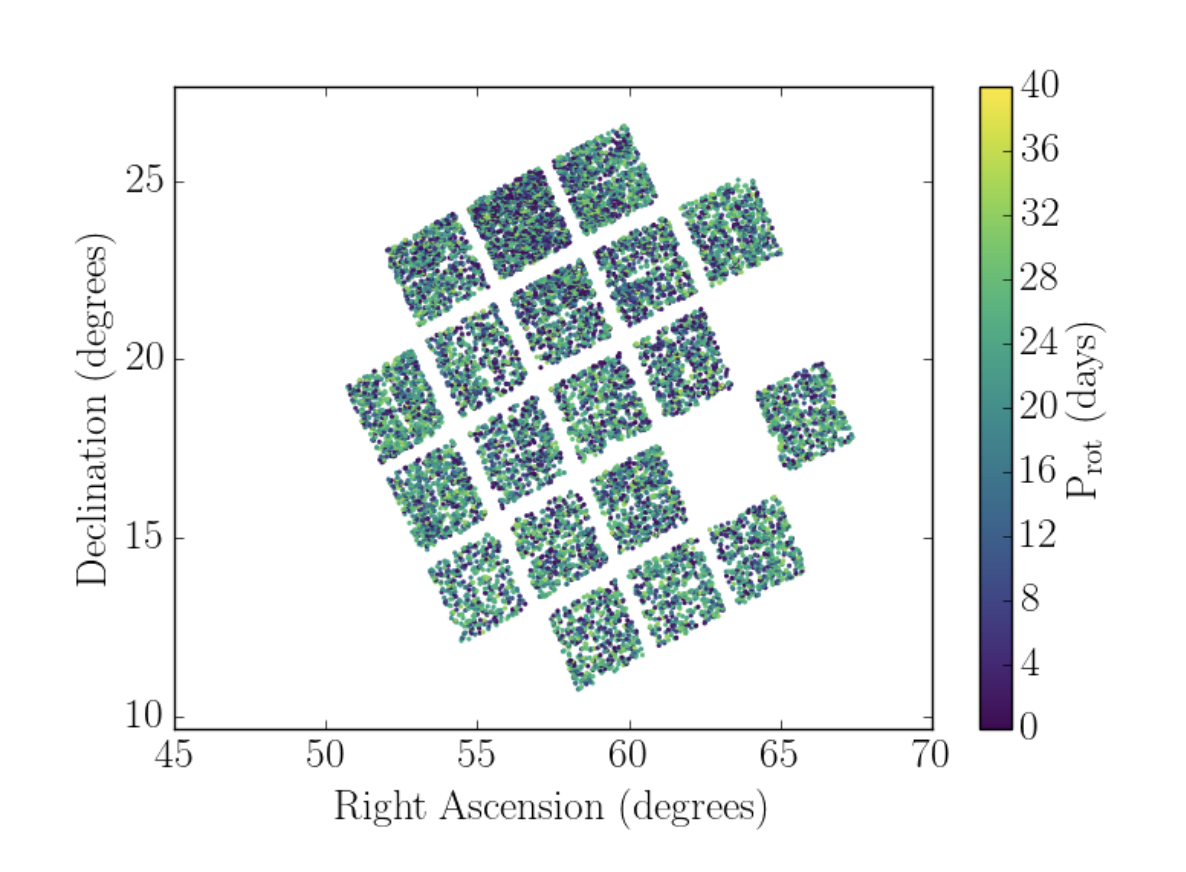
\includegraphics[width=6in, clip=true]{Kalesalad.png}
\caption{All stars observed during K2 campaign 4, plotted according to their
equatorial coordinates and colored by their preliminary rotation period.
These rotation periods were measured using a simple ACF method, applied to
    everest (Luger et al., 2015) light curves.}
\label{fig:kalesalad}
\end{center}
\end{figure}

We intend to measure rotation periods for all mid to low-mass dwarfs that show
evidence of rotational modulation in their light curves.

Need to measure rotation periods of all stars if you want to infer the
distribution of planets as a function of age.

It looks like hotter stars stop spinning down at around the age of the Sun.
However, that does not necessarily mean that gyrochronology cannot be used to
infer ages.
Gyro works for low mass stars down to around 0.35 M$_\odot$ (CITATION), up to
the age of the Universe.
It works for Solar-mass stars up to the age of the Sun and for stars more
massive than the Sun (but less massive than the Kraft break) it works to
gradually decreasing ages.
This means that X\% of stars in the TIC are likely to have ages that can be
determined by gyrochronology.

\section{Analysis Plan}

\section{Technical Feasibility}

\section{Expected Impact}

\section{Budget Justification}

\bibliographystyle{plainnat}
\bibliography{references}
\end{document}
